
\renewcommand{\EntradaBibtex}{ConteoLagartijas_UPV_2024}

\begin{frame}{\citetitle{\EntradaBibtex}$^*$ (1)}
\begin{block}{Motivación} 
El curl de bíceps es un ejercicio que se centra en fortalecer y desarrollar los músculos del bíceps braquial, contribuyendo a la fuerza y definición de los brazos
\begin{itemize}
\item Se implementó una aplicación móvil
\begin{itemize}
\item Permite al usuario llevar el conteo de las repeticiones que deben ser de frente y simulataneas
\item Debe ubicar el dispositivo a una distancia de 80 cm. 
\item Si se levanta las pesas de forma asimétrica, el conteo no se modifica.
\end{itemize}
\end{itemize}
\end{block} 

\footfullcite*{\EntradaBibtex}
\end{frame}


\begin{frame}{\citetitle{\EntradaBibtex} (2)}
%\begin{block}{Pantallas Principales} 
\begin{center}
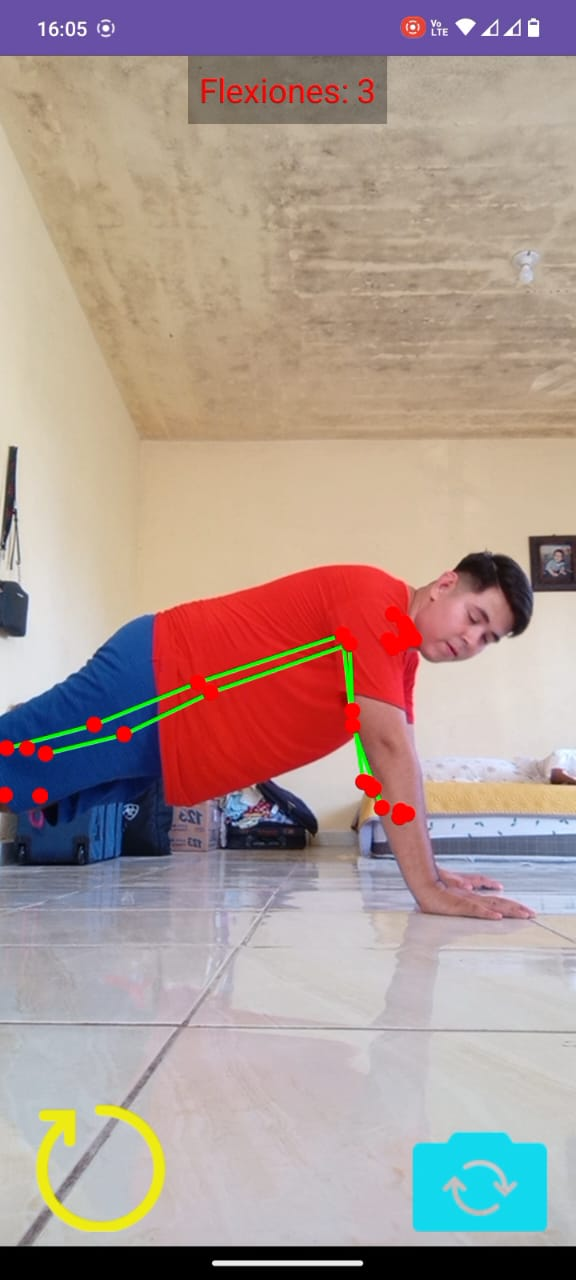
\includegraphics[width=0.40\linewidth]{2024_ConteoLagartijas/funcionamiento_app.png} 
\end{center}

\end{frame}


